\problemname{Infinity Issues}

After a long and stressful day at school, Bertha finally got home, but there is one thing she needs to do before she can have some fun.
You guessed right, she has to do homework.
Her task is to write a summary of ``The never ending story''.
Being a little special, Bertha thought she can at least have some fun while doing this.
She came up with the idea to write her summary on a never ending strip of paper. Funny, right?
Anyway, her desired result was to print the text on a single line.
Unfortunately, she has no printer which can handle infinite paper and standard A4 paper is not wide enough to fit her text in one line.

\begin{figure}[h]
	\centering
	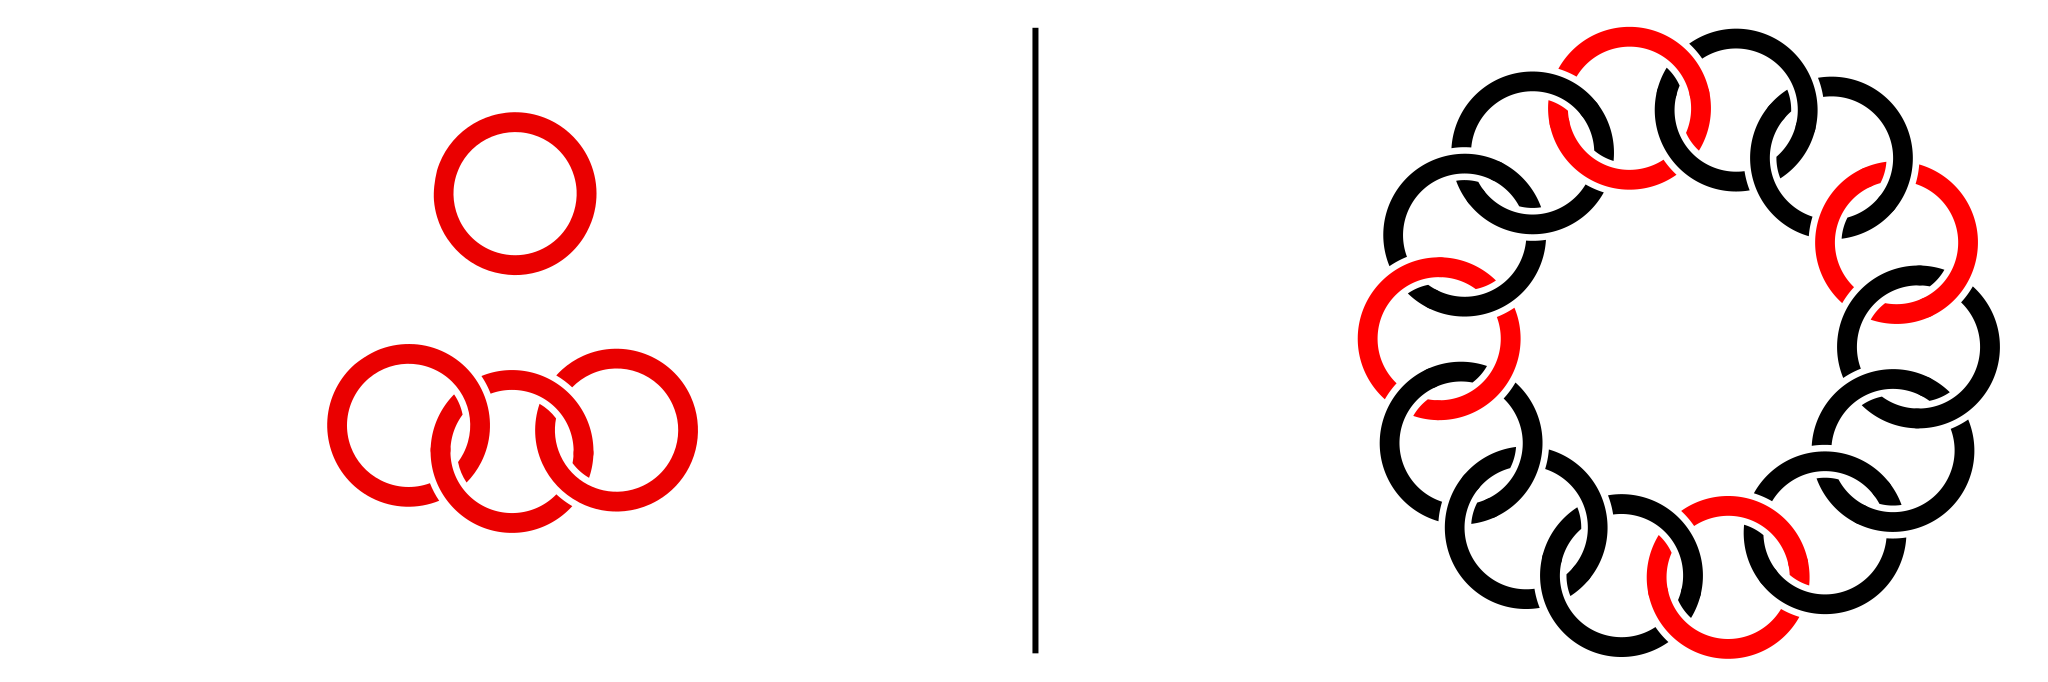
\includegraphics[width=0.75\linewidth]{example}
	\caption{A text written on a sheet of paper.
		The paper then was rolled up and glued together.
		And finally, it was cut into one long piece of paper.}
\end{figure}

However, Bertha had a brilliant idea, she could print the text in multiple lines of a single A4 sheet and glue the lines together.
She can simply glue the left and right sides of the paper together such that the end of line $i$ is at the start of line $i+1$ resulting in a slightly skewed cylinder where the text forms a continuous line.
If she additionally starts cutting below the line, she would end up with her desired strip of text.
However, there is one problem with that idea.
How should Bertha format her text such that the result looks like she intends?

\begin{Input}
    The input consists of:
    \begin{itemize}
        \item One line with two integers $n$ and $w$ ($1\leq n,w\leq 1000$), the number of words in your text and the number of characters that fit in one line.
        \item The next line contains $n$ lowercase words $s_i$ ($1\leq |s_i|\leq100$), the text you want to print.
        It is guaranteed that the words are separated by single spaces.
    \end{itemize}
\end{Input}

\begin{Output}
	Output the text such that printing it and gluing the page together as
	described above results in a text identical to the input.
	Note that whitespaces at the end of a line can be omitted or added, since this won't change the result.
	The same holds for new lines at the end of the text.
	Besides that, you need to print the text whitespace sensitive.
\end{Output}
